\documentclass[11pt,a4paper]{article}

\usepackage[a4paper,top=20mm,bottom=20mm,left=20mm,right=20mm,headsep=7mm,footskip=11mm]{geometry}
\usepackage{fontspec}
\usepackage{graphicx}
\usepackage{booktabs}
\usepackage{tabularx}
\usepackage{array}
\usepackage{xcolor}
\usepackage{hyperref}
\usepackage{float}

\setmainfont{Liberation Serif}
\setsansfont{Liberation Sans}
\setmonofont{Liberation Mono}

\definecolor{AgoraInk}{HTML}{172333}
\definecolor{AgoraMuted}{HTML}{5D6978}
\definecolor{AgoraTeal}{HTML}{168A8A}
\definecolor{AgoraCoral}{HTML}{E76F51}
\definecolor{AgoraGold}{HTML}{D99A2B}
\definecolor{AgoraBlue}{HTML}{427AA1}
\definecolor{AgoraPaleTeal}{HTML}{DCEEEE}
\definecolor{AgoraPaleCoral}{HTML}{F8E5DF}
\definecolor{AgoraPaleGold}{HTML}{F7EDDA}
\definecolor{AgoraLine}{HTML}{DCE3E8}
\definecolor{AgoraPaper}{HTML}{F7F9FA}

\hypersetup{
  colorlinks=true,
  linkcolor=AgoraTeal,
  urlcolor=AgoraBlue,
  pdftitle={Agora Comprehensive World Quality and Performance Evaluation},
  pdfauthor={Project Agora},
  pdfsubject={Blind qualitative review with objective generation and runtime evidence}
}

\setlength{\parindent}{0pt}
\setlength{\parskip}{5.5pt}
\setlength{\emergencystretch}{2em}
\renewcommand{\arraystretch}{1.22}
\newcolumntype{L}{>{\raggedright\arraybackslash}X}
\newcolumntype{R}{>{\raggedleft\arraybackslash}X}

\makeatletter
\renewcommand\section{\@startsection{section}{1}{0pt}%
  {2.1ex plus .4ex minus .2ex}{0.8ex}%
  {\color{AgoraInk}\sffamily\Large\bfseries}}
\renewcommand\subsection{\@startsection{subsection}{2}{0pt}%
  {1.6ex plus .3ex minus .2ex}{0.55ex}%
  {\color{AgoraTeal}\sffamily\large\bfseries}}
\renewcommand\subsubsection{\@startsection{subsubsection}{3}{0pt}%
  {1.2ex plus .2ex minus .1ex}{0.35ex}%
  {\color{AgoraInk}\sffamily\normalsize\bfseries}}
\def\ps@agora{
  \def\@oddhead{\sffamily\footnotesize\color{AgoraMuted}PROJECT AGORA\hfill COMPREHENSIVE WORLD EVALUATION}
  \def\@evenhead{\@oddhead}
  \def\@oddfoot{\sffamily\footnotesize\color{AgoraMuted}AUGUST 2026\hfill\thepage}
  \def\@evenfoot{\@oddfoot}
}
\makeatother
\pagestyle{agora}

\newcommand{\metric}[2]{%
  \colorbox{#1}{\parbox[c][18mm][c]{0.285\textwidth}{\centering\sffamily\color{AgoraInk}\textbf{#2}}}%
}
\newcommand{\scorepill}[3]{%
  \colorbox{#1}{\parbox[c][24mm][c]{0.285\textwidth}{%
    \centering\sffamily\color{AgoraInk}{\Large\bfseries #2}\\[-1pt]{\small #3}}}%
}
\newcommand{\band}[1]{\textsf{\textbf{#1}}}

\begin{document}

\begin{titlepage}
  \thispagestyle{empty}
  \vspace*{7mm}
  {\sffamily\small\bfseries\color{AgoraTeal}PROJECT AGORA \hfill EVALUATION REPORT 2026}

  \vspace{7mm}
  {\color{AgoraTeal}\rule{\textwidth}{2.2pt}}
  \vspace{17mm}

  {\sffamily\fontsize{31}{35}\selectfont\bfseries\color{AgoraInk}
    One Sentence, One World\par}
  \vspace{4mm}
  {\sffamily\fontsize{21}{26}\selectfont\color{AgoraInk}
    Comprehensive World Quality\par
    and Performance Evaluation\par}

  \vspace{9mm}
  {\sffamily\large\color{AgoraMuted}
    Blind dual-judge assessment combined with\par
    objective generation and runtime evidence}

  \vfill

  \noindent
  \scorepill{AgoraPaleTeal}{40\%}{Blind World Quality}\hfill
  \scorepill{AgoraPaleCoral}{35\%}{Objective Generation}\hfill
  \scorepill{AgoraPaleGold}{25\%}{Objective Runtime}

  \vspace{14mm}
  \colorbox{AgoraPaper}{%
    \parbox{0.94\textwidth}{%
      \vspace{4mm}
      \hspace{4mm}\begin{minipage}{0.88\textwidth}
      \sffamily\color{AgoraInk}
      \textbf{Evaluation thesis.} A high-quality world generator must do three things well:
      transform a single sentence into an imaginative social world, realize that world as a
      typed executable system, and sustain consequential behavior among agents and human
      participants. This report measures the complete path.
      \end{minipage}
      \vspace{4mm}
    }}

  \vspace{12mm}
  {\sffamily\small\color{AgoraMuted}Project Agora \hfill August 26, 2026}
\end{titlepage}

\section*{Executive View}

The evaluation combines human-readable world quality with hard evidence from generation,
compilation, and live execution. The result is a 0--100 score whose three partitions correspond
directly to Agora's central idea: language becomes a world, the world becomes executable, and
execution becomes a social process.

\vspace{2mm}
\noindent
\scorepill{AgoraPaleTeal}{86.10 / S}{GPT-5.6 Sol}\hfill
\scorepill{AgoraPaleCoral}{80.96 / A}{Gemini 3.7 Flash}\hfill
\scorepill{AgoraPaleGold}{98.8\%}{Within-one-tier agreement}

\vspace{4mm}
GPT-5.6 Sol establishes the current high-quality reference with the strongest blind world score
and objective generation result. Gemini 3.7 Flash forms a distinct second group through complete
first-pass generation, strong spatial and material imagination, and reliable execution. Gemini
3.1 Pro Preview and Gemini 2.5 Flash form a close third group with complementary strengths:
Pro is stronger in runtime interaction, while 2.5 Flash is stronger in objective generation.

Two advanced judges independently assessed the same anonymous worlds. Across 255 paired ratings,
ordinal Krippendorff's $\alpha$ is 0.801, quadratic-weighted $\kappa$ is 0.792, and 98.8\% of
judgments differ by at most one tier. The agreement gives the qualitative component a stable,
shared foundation while preserving meaningful differences between models.

\begin{figure}[H]
  \centering
  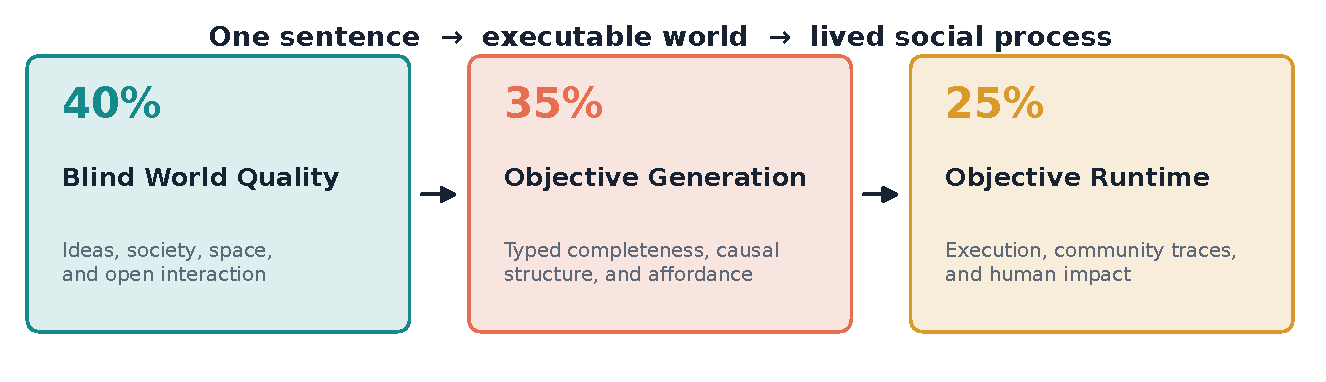
\includegraphics[width=\textwidth]{figures/evaluation_framework.pdf}
  \caption{The evaluation follows the system's full semantic path and assigns each stage a fixed share of the comprehensive score.}
\end{figure}

\clearpage
\section{Evaluation Idea}

World generation is more than producing a valid configuration. A world must embody its premise
through institutions, people, places, objects, and consequences. It must expose those ideas through
a typed representation that a coordinator can execute. Once running, it must respond to agents and
humans with causal continuity, spatial grounding, and meaningful state change.

The comprehensive score therefore joins three complementary forms of evidence:

\begin{center}
\metric{AgoraPaleTeal}{Blind quality: what kind of world was created?}\hfill
\metric{AgoraPaleCoral}{Generation: did the idea become an executable system?}\hfill
\metric{AgoraPaleGold}{Runtime: what happens when the world is inhabited?}
\end{center}

\vspace{2mm}
The fixed aggregation is
\[
  \mathrm{Comprehensive}
  = 0.40\,Q_{\mathrm{blind}}
  + 0.35\,G_{\mathrm{objective}}
  + 0.25\,R_{\mathrm{objective}}.
\]
Blind world quality receives the largest share because the task begins with imagination: the
one-sentence premise must become a distinctive social possibility space. Objective generation
then verifies that these ideas exist in a complete executable world. Objective runtime measures
the lived process produced by that world.

\subsection{Score Bands}

The bands make the 0--100 allocation easy to read while leaving the underlying numeric score intact.

\begin{center}
\small
\begin{tabular}{cccccc}
\toprule
\band{S} & \band{A} & \band{B} & \band{C} & \band{D} & \band{E} \\
85--100 & 80--84.99 & 70--79.99 & 60--69.99 & 40--59.99 & 0--39.99 \\
\bottomrule
\end{tabular}
\end{center}

\section{Method and Standards}

\subsection{Blind World Quality: 40\%}

Gemini 3.1 Pro Preview and GPT-5.6 Sol independently evaluated anonymous evidence from the same
generated worlds. Model names, prior scores, costs, latencies, and objective metrics were absent
from the review material. Each compiled world appeared in three separately shuffled panels per
dimension for each judge, yielding six ratings for every world--dimension pair.

The judges assigned an absolute tier from 0 to 6 rather than ranking candidates. The aggregation
takes the median of six tier-derived scores for each world and dimension, averages across three
matched source premises, and applies the fixed quality weights below.

\begin{table}[htbp]
\centering
\small
\begin{tabularx}{\textwidth}{@{}L r L@{}}
\toprule
\textbf{Dimension} & \textbf{Weight} & \textbf{Standard} \\
\midrule
Premise and causal institutions & 25.81\% & The sentence becomes a specific system of institutions, state variables, feedback, and stakes. \\
Society and personhood & 23.66\% & Groups and named people possess distinct goals, leverage, dependencies, relationships, and material lives. \\
Space and materiality & 10.75\% & Places and objects are world-specific, readable, and necessary to the premise. \\
Open-ended interaction & 32.26\% & Humans and agents can pursue different strategies, including coordinator-checked actions beyond a fixed catalog. \\
Holistic coherence & 7.53\% & The parts form a distinctive world that invites continued exploration. \\
\bottomrule
\end{tabularx}
\end{table}

\subsection{Objective Generation: 35\%}

Objective generation joins contract compliance with measurable world structure. Contract compliance
measures complete typed output, compilation, required populations, locations, items, actions, and
player affordances. Objective world quality measures ten structural axes:

\begin{center}
\small\sffamily\color{AgoraInk}
causal system \quad spatial necessity \quad agent individuation \quad social interdependence\\
material economy \quad interaction depth \quad human affordance \quad template escape\\
visual authorship \quad first-pass robustness
\end{center}

The resulting score rewards worlds that are simultaneously imaginative, complete, and executable.
Compiled-world coverage and first-pass completion remain visible beside the aggregate so that the
score reflects both semantic depth and dependable realization.

\subsection{Objective Runtime: 25\%}

Objective runtime executes generated worlds under matched interventions and human events. It combines
execution compliance, strict trace quality, and cross-world stress performance. Trace quality spans:

\begin{center}
\small\sffamily\color{AgoraInk}
intervention sensitivity \quad causal threading \quad role conditioning \quad open-action substance\\
state evolution \quad social differentiation \quad human impact \quad conflict and recovery\\
behavioral specificity \quad spatial causality
\end{center}

This partition measures whether authored institutions and affordances become observable behavior:
agents respond to new events, proposals create world state changes, actions remain role- and
place-sensitive, and human participation becomes part of the causal trace. A model that produces no
executable generated world receives zero for the end-to-end runtime partition.

\subsection{System Claim to Evidence Alignment}

Each score partition corresponds to a concrete part of the system proposition. The alignment keeps
the comprehensive result conceptually direct: every point represents either world quality,
executable realization, or behavior inside the generated world.

\begin{table}[H]
\centering
\small
\begin{tabularx}{\textwidth}{@{}L L L@{}}
\toprule
\textbf{Agora proposition} & \textbf{Primary evidence} & \textbf{What earns a high score} \\
\midrule
One sentence becomes one world & Blind dual-judge quality & Distinctive premise transformation, social organization, material specificity, and open possibility. \\
The world is executable & Objective generation & Complete typed output, causal and spatial structure, player affordances, and robust compilation. \\
The world becomes inhabited & Objective runtime & Responsive traces, state evolution, role-sensitive action, human impact, and spatial causality. \\
\bottomrule
\end{tabularx}
\end{table}

\clearpage
\section{Comprehensive Scores}

\begin{figure}[H]
  \centering
  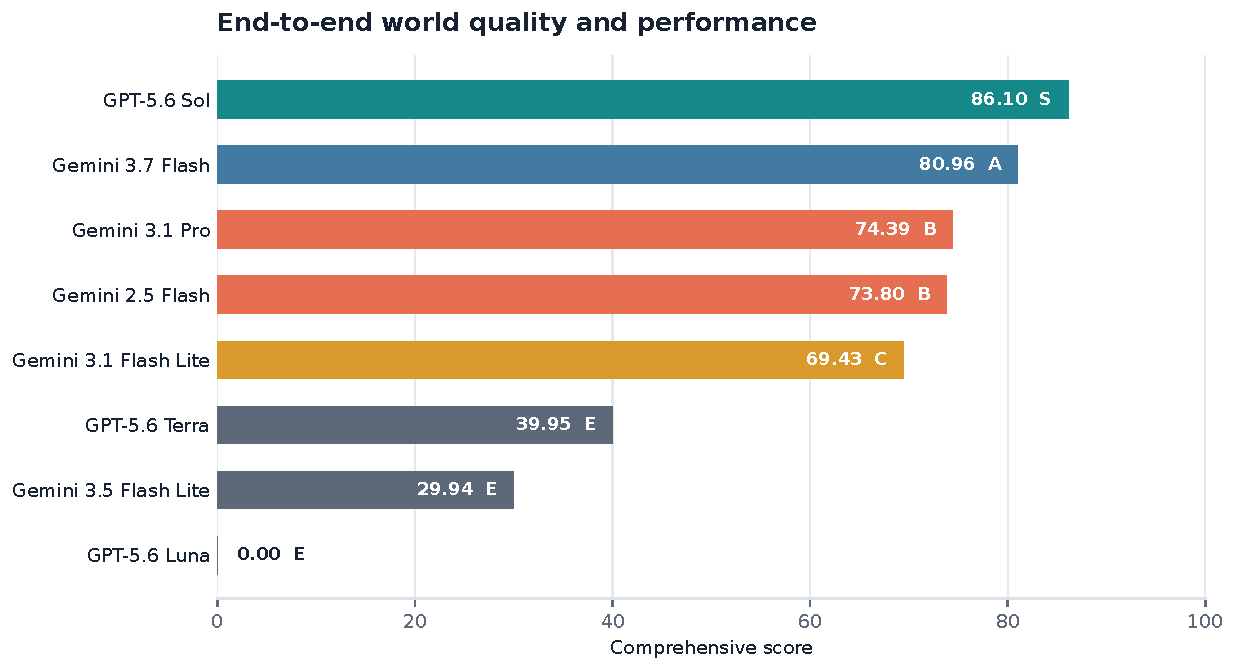
\includegraphics[width=0.91\textwidth]{figures/comprehensive_scores.pdf}
  \caption{The comprehensive score produces a wide, readable distribution across end-to-end capability levels.}
\end{figure}

\begin{table}[H]
\centering
\footnotesize
\begin{tabularx}{\textwidth}{@{}Lrrrrrr@{}}
\toprule
\textbf{Model} & \textbf{Blind} & \textbf{Generation} & \textbf{Runtime} & \textbf{Total} & \textbf{Band} & \textbf{Compiled} \\
\midrule
Gemini 2.5 Flash & 62.04 & 87.71 & 73.13 & \textbf{73.80} & \band{B} & 3/3 \\
Gemini 3.1 Flash Lite & 57.53 & 85.01 & 66.64 & \textbf{69.43} & \band{C} & 3/3 \\
Gemini 3.1 Pro Preview & 64.95 & 81.72 & 79.23 & \textbf{74.39} & \band{B} & 3/3 \\
Gemini 3.5 Flash Lite & 20.91 & 28.25 & 46.74 & \textbf{29.94} & \band{E} & 1/3 \\
Gemini 3.7 Flash & 78.96 & 88.20 & 74.04 & \textbf{80.96} & \band{A} & 3/3 \\
GPT-5.6 Luna & 0.00 & 0.00 & 0.00 & \textbf{0.00} & \band{E} & 0/3 \\
GPT-5.6 Sol & 85.00 & 92.15 & 79.40 & \textbf{86.10} & \band{S} & 3/3 \\
GPT-5.6 Terra & 27.47 & 29.87 & 74.01 & \textbf{39.95} & \band{E} & 1/3 \\
\bottomrule
\end{tabularx}
\end{table}

The allocation forms distinct performance groups. GPT-5.6 Sol reaches the S band through the
strongest blind world quality and objective generation score together with top-tier runtime behavior.
Gemini 3.7 Flash forms the A band with strong premise transformation, spatial-material realization,
and generation reliability. Gemini 3.1 Pro Preview and Gemini 2.5 Flash occupy the B band through
different strengths, and Gemini 3.1 Flash Lite forms the C band as a capable complete-world generator.

\begin{figure}[H]
  \centering
  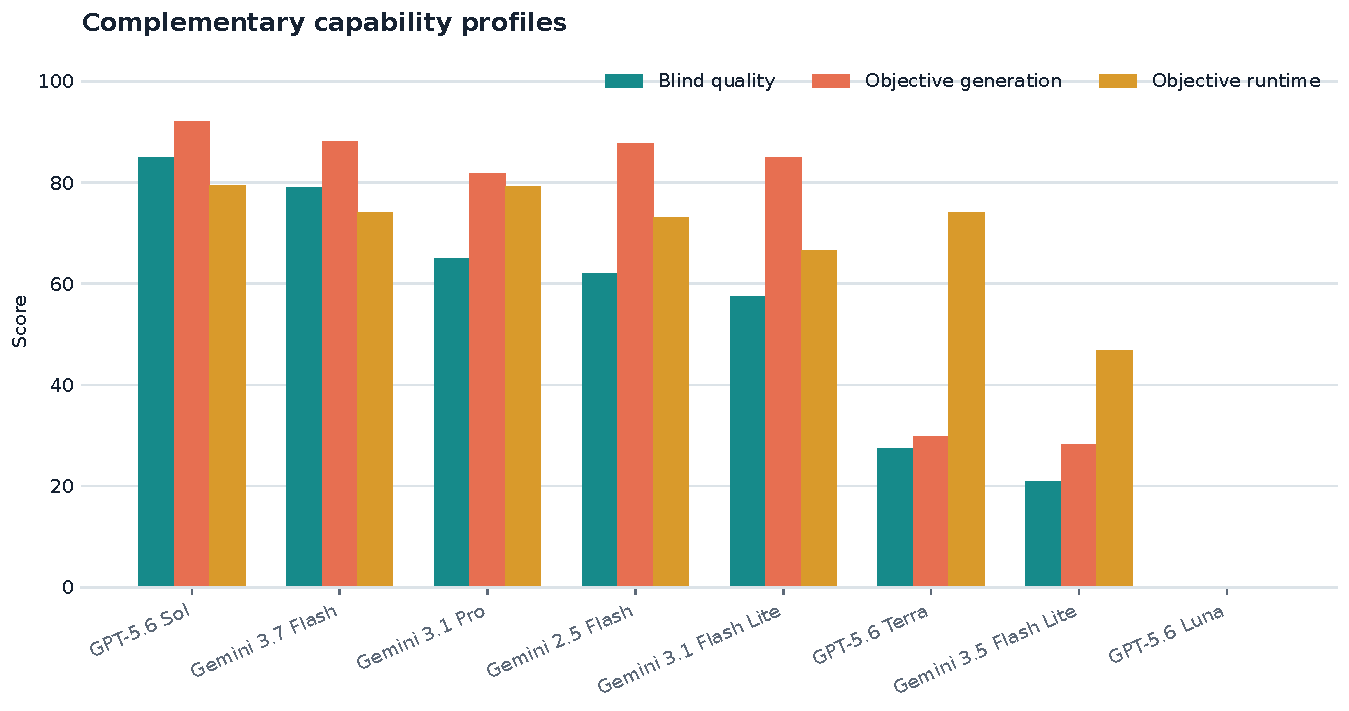
\includegraphics[width=\textwidth]{figures/partition_profile.pdf}
  \caption{The three partitions reveal complementary model profiles rather than a one-dimensional quality ordering.}
\end{figure}

\section{Blind World Quality}

The qualitative dimensions produce a meaningful spread without collapsing distinct skills. GPT-5.6
Sol sustains an 85-level result across every category. Gemini 3.7 Flash is strongest in premise
transformation and spatial-material realization. Gemini 3.1 Pro Preview and Gemini 2.5 Flash separate
through different profiles, while Gemini 3.1 Flash Lite remains competitive in space and interaction.

\begin{figure}[H]
  \centering
  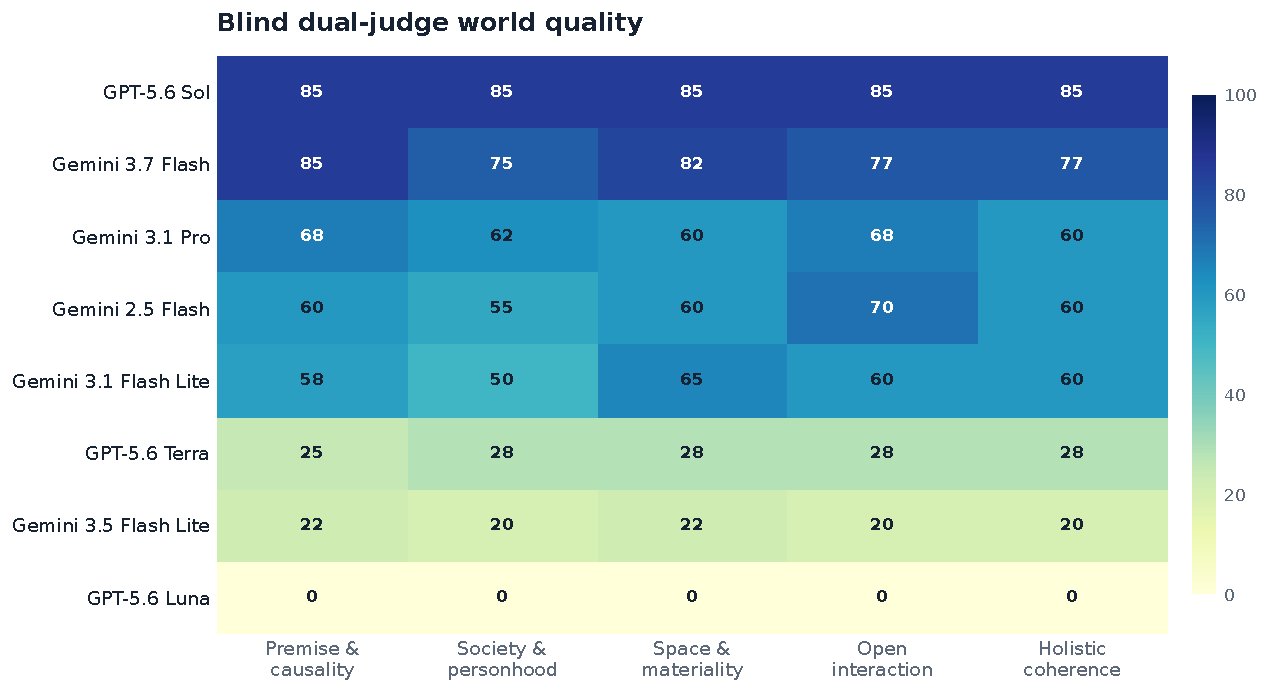
\includegraphics[width=0.92\textwidth]{figures/quality_heatmap.pdf}
  \caption{Dual-judge quality scores across the five dimensions. Generation coverage remains part of the matched-premise aggregate.}
\end{figure}

\begin{table}[H]
\centering
\scriptsize
\begin{tabularx}{\textwidth}{@{}Lrrrrrr@{}}
\toprule
\textbf{Model} & \textbf{Quality} & \textbf{Premise} & \textbf{Society} & \textbf{Space} & \textbf{Interaction} & \textbf{Holistic} \\
\midrule
Gemini 2.5 Flash & \textbf{62.04} & 60.00 & 55.00 & 60.00 & 70.00 & 60.00 \\
Gemini 3.1 Flash Lite & \textbf{57.53} & 57.50 & 50.00 & 65.00 & 60.00 & 60.00 \\
Gemini 3.1 Pro Preview & \textbf{64.95} & 67.50 & 62.50 & 60.00 & 67.50 & 60.00 \\
Gemini 3.5 Flash Lite & \textbf{20.91} & 22.50 & 20.00 & 22.50 & 20.00 & 20.00 \\
Gemini 3.7 Flash & \textbf{78.96} & 85.00 & 75.00 & 81.67 & 76.67 & 76.67 \\
GPT-5.6 Luna & \textbf{0.00} & 0.00 & 0.00 & 0.00 & 0.00 & 0.00 \\
GPT-5.6 Sol & \textbf{85.00} & 85.00 & 85.00 & 85.00 & 85.00 & 85.00 \\
GPT-5.6 Terra & \textbf{27.47} & 25.00 & 28.33 & 28.33 & 28.33 & 28.33 \\
\bottomrule
\end{tabularx}
\end{table}

\subsection{Inter-Judge Consistency}

The two judges agree on both the broad model structure and the individual quality dimensions.
Overall ordinal $\alpha=0.801$, weighted $\kappa=0.792$, and tier-score correlation is 0.780.
Exact tier agreement is 60.4\%; within-one-tier agreement reaches 98.8\%. The average severity
difference between the two judges is 2.29 points.

\begin{figure}[H]
  \centering
  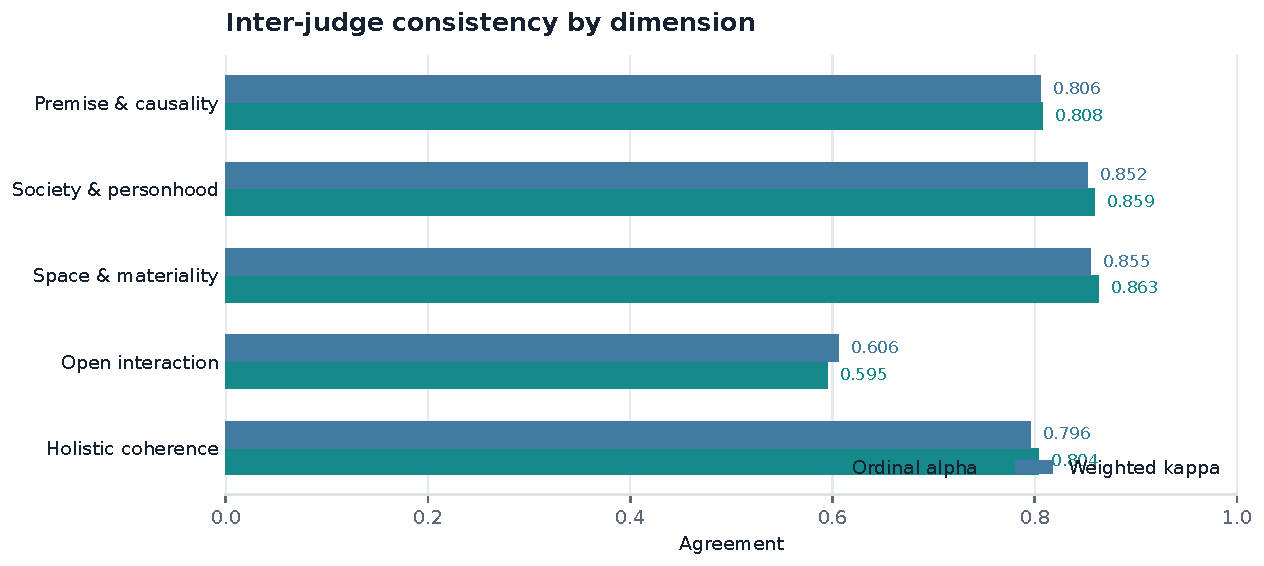
\includegraphics[width=0.88\textwidth]{figures/judge_agreement.pdf}
  \caption{Independent agreement remains high across the conceptual, social, spatial, interactive, and holistic dimensions.}
\end{figure}

Agreement is strongest for spatial and material imagination, society and personhood, premise
transformation, and holistic coherence. Open-ended interaction generates the widest range of
interpretation because it asks judges to infer future behavior from a finite world specification;
even there, 94.1\% of paired ratings remain within one tier.

\clearpage
\section{Objective Generation}

Objective generation sharply separates complete world builders from partial outputs. GPT-5.6 Sol
combines the deepest causal and material structures with the highest human affordance. Gemini 3.7
Flash leads first-pass robustness. Gemini 2.5 Flash combines strong agent individuation, material
economy, interaction depth, and human affordance. The scores reward both semantic richness and
successful realization under the common typed contract.

\begin{figure}[H]
  \centering
  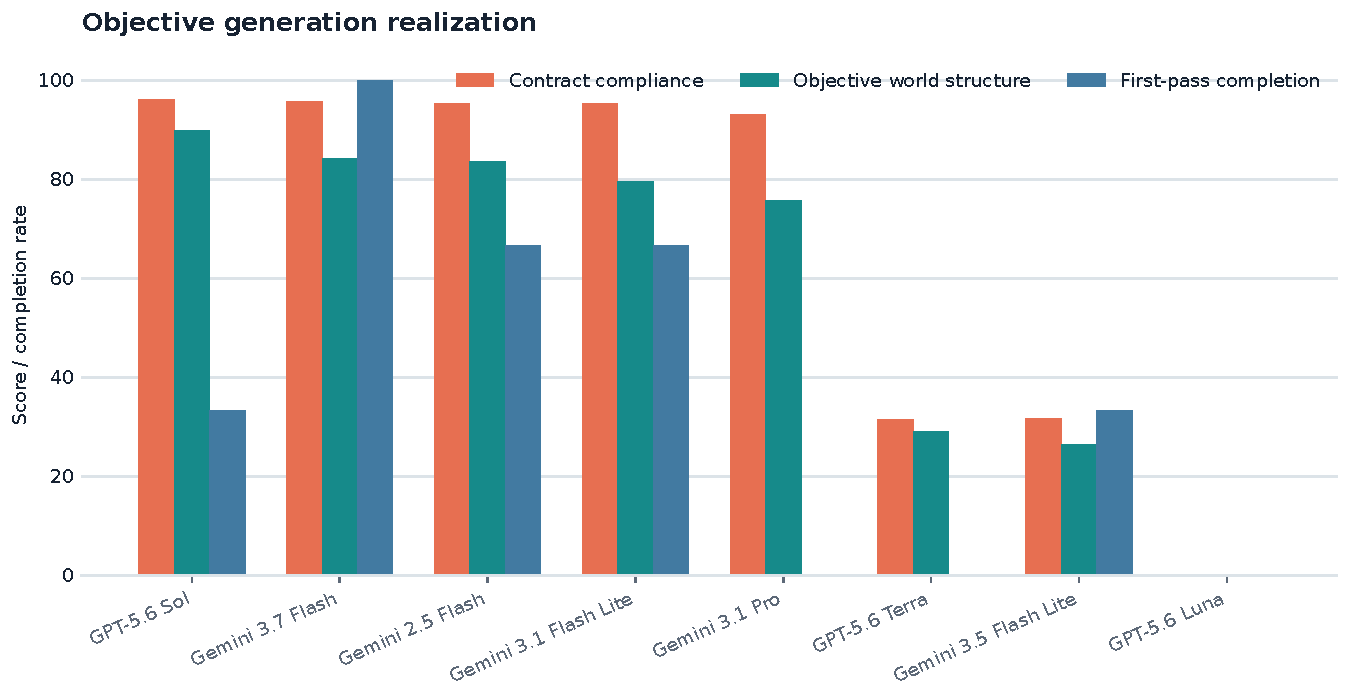
\includegraphics[width=\textwidth]{figures/generation_components.pdf}
  \caption{Contract compliance, objective world structure, and first-pass completion reveal how models realize authored ideas.}
\end{figure}

\begin{table}[H]
\centering
\small
\begin{tabularx}{\textwidth}{@{}Lrrrr@{}}
\toprule
\textbf{Model} & \textbf{Generation} & \textbf{Contract} & \textbf{World structure} & \textbf{First pass} \\
\midrule
Gemini 2.5 Flash & \textbf{87.71} & 95.25 & 83.67 & 2/3 \\
Gemini 3.1 Flash Lite & \textbf{85.01} & 95.35 & 79.61 & 2/3 \\
Gemini 3.1 Pro Preview & \textbf{81.72} & 93.19 & 75.81 & 0/3 \\
Gemini 3.5 Flash Lite & \textbf{28.25} & 31.66 & 26.47 & 1/3 \\
Gemini 3.7 Flash & \textbf{88.20} & 95.75 & 84.16 & 3/3 \\
GPT-5.6 Luna & \textbf{0.00} & 0.00 & 0.00 & 0/3 \\
GPT-5.6 Sol & \textbf{92.15} & 96.17 & 89.93 & 1/3 \\
GPT-5.6 Terra & \textbf{29.87} & 31.41 & 29.02 & 0/3 \\
\bottomrule
\end{tabularx}
\end{table}

\section{Objective Runtime}

Runtime scoring reveals a complementary capability axis. GPT-5.6 Sol and Gemini 3.1 Pro Preview
produce the strongest overall operational performance. Gemini 2.5 Flash achieves the highest strict
trace quality through substantive open proposals, causal threading, and human uptake. Gemini 3.7
Flash contributes highly reliable execution and intervention sensitivity. The partition recognizes
multiple successful styles of community behavior instead of collapsing them into an action count.

\begin{figure}[H]
  \centering
  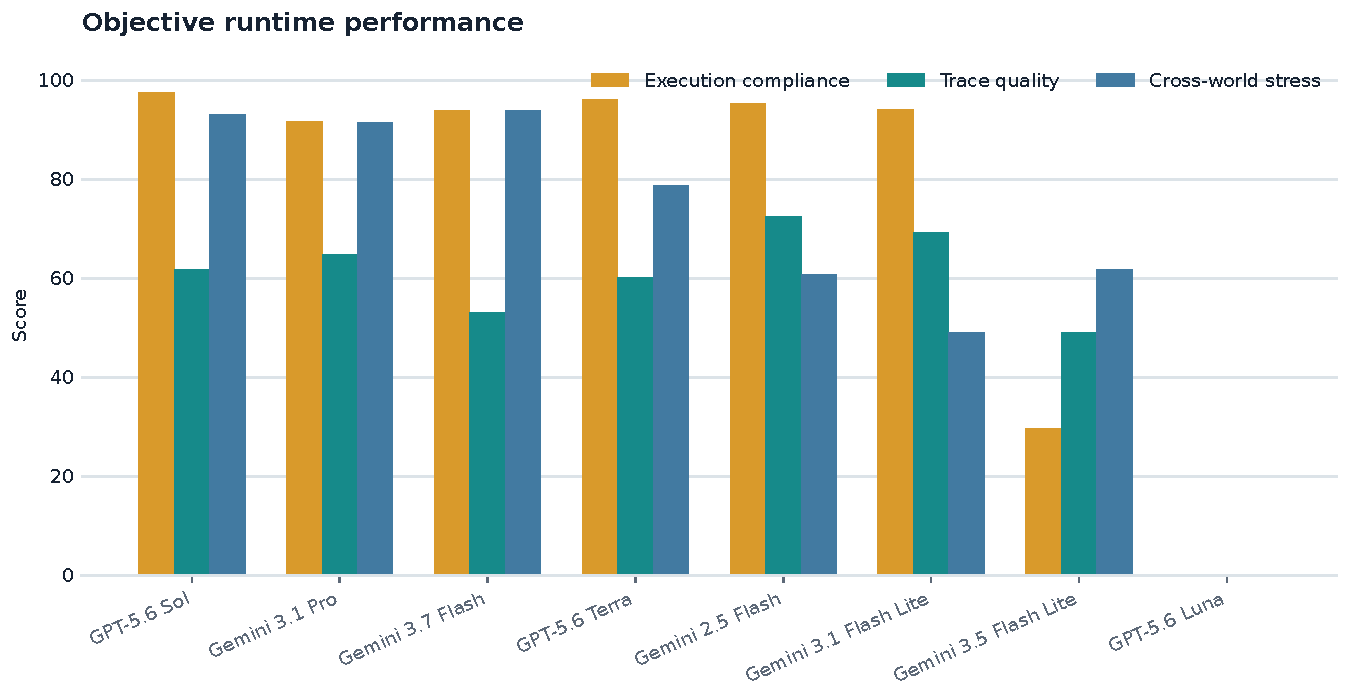
\includegraphics[width=\textwidth]{figures/runtime_components.pdf}
  \caption{Runtime performance combines successful execution, trace substance, and behavior across generated worlds.}
\end{figure}

\begin{table}[H]
\centering
\small
\begin{tabularx}{\textwidth}{@{}Lrrrr@{}}
\toprule
\textbf{Model} & \textbf{Runtime} & \textbf{Execution} & \textbf{Trace quality} & \textbf{Cross-world} \\
\midrule
Gemini 2.5 Flash & \textbf{73.13} & 95.31 & 72.41 & 60.70 \\
Gemini 3.1 Flash Lite & \textbf{66.64} & 94.03 & 69.32 & 49.00 \\
Gemini 3.1 Pro Preview & \textbf{79.23} & 91.59 & 64.72 & 91.50 \\
Gemini 3.5 Flash Lite & \textbf{46.74} & 29.74 & 49.00 & 61.84 \\
Gemini 3.7 Flash & \textbf{74.04} & 93.86 & 53.11 & 93.87 \\
GPT-5.6 Luna & \textbf{0.00} & 0.00 & 0.00 & 0.00 \\
GPT-5.6 Sol & \textbf{79.40} & 97.54 & 61.83 & 93.03 \\
GPT-5.6 Terra & \textbf{74.01} & 96.15 & 60.23 & 78.67 \\
\bottomrule
\end{tabularx}
\end{table}

\clearpage
\section{Integrated Reading}

The combined evaluation produces both agreement and separation. The blind judges agree on the broad
quality structure, while the hard metrics explain why worlds with similar conceptual appeal diverge
once compilation and runtime behavior are included. A high comprehensive score requires strength
across all three stages: world imagination, executable realization, and lived interaction.

\vspace{2mm}
\colorbox{AgoraPaleTeal}{%
  \parbox{0.96\textwidth}{%
    \vspace{3mm}\hspace{3mm}\begin{minipage}{0.91\textwidth}
    \sffamily\color{AgoraInk}
    \textbf{S band -- GPT-5.6 Sol.} The strongest world quality and objective generation result,
    joined with leading execution compliance and human impact. Its worlds establish the current
    high-quality reference for the suite.
    \end{minipage}\vspace{3mm}}}

\vspace{3mm}
\colorbox{AgoraPaleCoral}{%
  \parbox{0.96\textwidth}{%
    \vspace{3mm}\hspace{3mm}\begin{minipage}{0.91\textwidth}
    \sffamily\color{AgoraInk}
    \textbf{A band -- Gemini 3.7 Flash.} Strong blind quality, complete first-pass generation,
    reliable execution, and a distinctive spatial-material profile produce a clear second group.
    \end{minipage}\vspace{3mm}}}

\vspace{3mm}
\colorbox{AgoraPaleGold}{%
  \parbox{0.96\textwidth}{%
    \vspace{3mm}\hspace{3mm}\begin{minipage}{0.91\textwidth}
    \sffamily\color{AgoraInk}
    \textbf{B and C bands -- differentiated complete-world generators.} Gemini 3.1 Pro Preview
    leads in runtime interaction, Gemini 2.5 Flash in objective generation and trace quality, and
    Gemini 3.1 Flash Lite in efficient complete-world coverage with solid open interaction.
    \end{minipage}\vspace{3mm}}}

\vspace{5mm}
The score allocation is broad and interpretable. Quality judgment establishes whether the world is
worth entering; generation metrics establish whether its ideas are structurally realized; runtime
metrics establish whether those structures produce consequential behavior. Together they evaluate
the defining Agora proposition: \textbf{one sentence becomes one executable, inhabited world}.

\vfill
\begin{center}
  {\color{AgoraLine}\rule{0.72\textwidth}{0.6pt}}\\[4mm]
  {\sffamily\small\color{AgoraMuted}PROJECT AGORA \quad ONE SENTENCE, ONE WORLD}
\end{center}

\end{document}
